

\documentclass[2dCFT-lecture.tex]{subfiles}


\begin{document}

\setcounter{tocdepth}{2}
%\maketitle
\section{Minimal Models}
This chapter is devoted to particularly simple conformal theory called \textbf{minimal models} first studied in the seminal paper \cite[ISZ88-No.1]{belavin1984infinite}. These theories
are characterized by a Hilbert space made of a finite numbers of representations of the Verma modules.

\subsection{Conformal Family}
From the previous study, we know that primary fields
play a fundamental role in conformal field theory. The
asymptotic state is given by $\ket{h}=\phi(0)\ket{0}$,
which satisfies $L_0 \ket{h}=h\ket{h}$ and $L_n \ket{h}=0$ for  $n>0$. In Verma module section, we also defined descendant states leading by primary $\ket{h}$, by acting a series of $L_{-n}$ on $\ket{h}$.
We first study the field operator corresponding to the
descendant states. The natural definition of the
descendant field associated with the state $L_{-n}\ket{h}$ is

\begin{equation}
\label{def-descendant-field}
\phi^{(- n) } (w) \equiv \left(L _{- n } \phi \right) (w)=\frac{1 }{2 \pi i } \oint _{w } d z \frac{1 }{(z-w)^{n-1 } } T (z) \phi (w)\, .
\end{equation}
By using the OPE \eqref{OPE-T-primaryfield-z}, we
can the above expression can be calculated explicitly.
In particular, we have
\begin{equation}
 \phi^{(0) } (w)=h \phi (w)\, , \quad \text{and } \quad \phi^{(- 1) } (w)=\partial \phi (w)\, .
\end{equation}
Now consider the correlation function with one descendant field in it, i.e.
\begin{equation}
  \left\langle \left(L _{- n } \phi \right) (w) X \right\rangle\, ,
\end{equation}
where $X=\phi _{1 } \left(w _{1 } \right) \cdots \phi _{N } \left(w _{N } \right)$ is a
product of primary fields with conformal dimensions $h_i$.
This correlation function can be calculated by substituting the definition \eqref{def-descendant-field}.

\bea
\label{differential-equation}
 \left\langle \phi^{(- n) } (w) X \right\rangle
 &= \frac{1 }{2 \pi i } \oint _{w } d z (z-w)^{1-n } \langle T (z) \phi (w) X \rangle\notag \\
 &=- \frac{1 }{2 \pi i } \oint _{\left(w _{i } \right) } d z (z-w)^{1-n } \sum _{i } \{\frac{1 }{z-w _{i } } \partial _{w _{i } } \langle \phi (w) X \rangle+ \frac{h _{i } }{\left(z-w _{i } \right)^{2 } } \langle \phi (w) X \rangle \}\notag \\
 &\equiv \mathcal{L } _{- n } \langle \phi (w) X \rangle \quad (n \geq 1)\, .
\eea

In the second step, the residue theorem is applied by
reversing the contour including $w$ only and summing
the contributions from all the poles at $w_i$. With
the help of the relevant OPEs, the definition operator $\mathcal{L }_{-n}$ is given by
\begin{equation}
 \mathcal{L } _{- n }=\sum _{i } \left\{\frac{(n-1) h _{i } }{\left(w _{i }-w \right)^{n } }-\frac{1 }{\left(w _{i }-w \right)^{n-1 } } \partial _{w _{i } } \right\}\, .
\end{equation}
This result tells us that the evaluation of a correlation function containing one descendant field
$\phi^{(-n)}$ is controlled by its primary field. $\mathcal{L}_{-1}$ is equivalent to $\partial/\partial{w}$, since the operator
\begin{equation}
\frac{\partial }{\partial w } + \sum _{i } \frac{\partial }{\partial w _{i } }\, ,
\end{equation}
annihilates any correlation functions because of the translation invariance.

The descendant states corresponding to $L_{-k}L_{-n}\ket{h}$ can be defined recursively.
\begin{equation}
\phi^{(- k ,-n) } (w) \equiv \left(L _{- k } L _{- n } \phi \right) (w)
=  \frac{1 }{2 \pi i } \oint _{w } d z (z-w)^{1-k } T (z) \left(L _{- n } \phi \right) (w)\, .
\end{equation}
In particular, we have
\begin{equation}
\phi^{(0 ,-n) } (w)=(h + n) \phi^{(- n) } (w) \quad \text{and} \quad
\phi^{(- 1 ,-n) } (w)=\partial _{w } \phi^{(- n) } (w)\, .
\end{equation}
And it can be shown directly that
\begin{equation}\label{eq-BPZ}
\left\langle \phi^{\left(- k _{1 } \ldots \ldots-k _{n } \right) } (w) X \right\rangle=\mathcal{L } _{- k _{1 } } \cdots \mathcal{L } _{- k _{n } } \langle \phi (w) X \rangle\, .
\end{equation}
That is nothing but to apply the differential operators in succession. Consequently, correlation
functions of descendant fields attributes to correlation functions of primary field.  If we obtain all the correlation functions of primary fields in a theory, then the correlation functions including descendant fields are thus all determined.

Moreover, all the OPEs with $T(z)$ with descendant states can be calculated in a similar fashion. For example, for
$\phi^{(-1)}=\partial\phi$
\bea
T(z)\partial\phi(w)&\sim \frac{2h\phi(w)}{(z-w)^3}
+\frac{(h+1)\partial\phi(w)}{(z-w)^2}
+\frac{\partial^2\phi(w)}{z-w}\notag\\
&\sim\frac{2\phi^{(0)}(w)}{(z-w)^3}
+\frac{(h+1)\phi^{(-1)}(w)}{(z-w)^2}
+\frac{\phi^{(-1,-1)}(w)}{z-w}\, ,
\eea
where we have neglect the regular terms as usual.
The set of a primary field $\phi$
and all of its descendants is called the \textbf{conformal family} of $\phi$, denoted by $[\phi]$. The OPEs with $T(z)$ are closed in the conformal family.





\subsection{Minimal models}\label{sec:MM}
In a conformal field theory (or more generally quantum field theories),
we want to understand correlation functions in the
theory. For free bosons and fermions,
all correlation functions can be calculated by directly using partition function.
However, it is not so straightforward to determine all the correlation functions for the interacting CFTs.
If there are only finitely many  highest weight representations of Virasoro algebra (or finitely many primary fields), one can perform exact computations of correlation functions \cite[ISZ88-No.1]{belavin1984infinite}. Such CFTs are called \textbf{minimal models}.  Let us consider a theory with the set of finitely many highest
weights $\{h_1,\cdots h_p\}$ so that OPEs take the following form:
\begin{equation}\label{op-algebra}
\phi _{1 } (z , \overline{z}) \phi _{2 } (0,0)
=\sum_p \sum_{\{k,\overline k\}} C^{p\{k,\overline k\}}_{12}
z^{h _{p }-h _{1 }-h _{2 } + K } \overline{z } ^{\overline{h } _{p }-\overline{h } _{1 }-\overline{h } _{2 } + \overline{K } }
\phi^{\{k,\overline{k}\}}_p(0,0)\, ,
\end{equation}
where $K=\sum_i k_i$ and $\overline{K }=\sum_i \overline{k}_i$, and $\phi_{i}$ is the primary field with
highest weight $h_i$. As we have seen in the last subsection,  all the correlation function can be
reduced to the correlation function constructed by
primary fields. Hence, we just need to understand OPEs of primary fields in minimal models, and we do not need a concrete realization of the CFT. In this section, we will determine OPEs of primary fields in the minimal models.


\subsubsection*{Kac Determinant}

A representation
of the Virasoro algebra is said to be unitary if it contains no negative-norm states.
In the section of Verma module, we have mentioned
that the negative of central charge and highest weight
will make the states non-unitary.
As we will see below, the unitarity
imposes strong constraints on $(h,c)$.

In addition to unitarity, one has to pay attention to zero-norm states, indeed.
If a state $|\chi\rangle$ in a Verma module $V(c,h)$ which is not a highest weight state satisfies the condition
$$
L_n|\chi\rangle=0~, \quad \textrm{for} ~ n>0~,
$$
it is called a \textbf{singular vector}. In fact, a singular vector $|\chi\rangle$ is orthogonal to any state $\prod_i L_{-n_i}|h\rangle$ in the Verma module $V(c,h)$
$$
\langle \chi| \prod_{i}L_{-n_i}|h\rangle=0~.
$$
Therefore, the norm of a singular vector is zero; $\langle\chi|\chi\rangle=0$ so that it is also called a \textrm{null vector} or a \textrm{null state}.

Suppose that there exists a singular vector $|\chi\rangle$ at level $N$ in the Verma module, namely $L_0|\chi\rangle=(h+N)|\chi\rangle$. Then 	its descendants
$$
	L_{-k_1}L_{-k_2}\cdots L_{-k_n}\ket{\chi}\, ,
	\qquad (1\leq k_1 \leq k_2 \cdots \leq k_n)
$$
are all null, and moreover they form a submodule in the Verma module $V(c,h)$. Therefore, in this situation the Verma module is \textbf{reducible}. In fact, the Verma module $V(c,h)$ is irreducible if and only if it contains no singular vector. Otherwise, an irreducible representation of the Virasoro algebra is
$$
L(c,h)=V(c,h)/J(c,h)
$$
where $J(c,h)$ consists of all null states and their descendants
$$
J(c,h)=\bigcup_{\chi:\textrm{null}}~ \{L_{-k_1}L_{-k_2}\cdots L_{-k_n}\ket{\chi}\}	\qquad (1\leq k_1 \leq k_2 \cdots \leq k_n)
~.
$$



To see a Verma module has a null state, let us define a Gram matrix as matrix element
$M_{ij}=\bra{i}\ket{j}$. $\ket{i},\ket{j}$ are basis.
For instance, at level two, we have 2 basis
$L_{-2}\ket{h}$, $L_{-1}^2\ket{h}$.
Therefore, the Gram matrix is
\bea
\left(\begin{array}{c c }{\left\langle h \left| L _{2 } L _{- 2 } \right| h \right\rangle } &{\left\langle h \left| L _{1 }^{2 } L _{- 2 } \right| h \right\rangle } \\{\left\langle h \left| L _{2 } L _{- 1 }^{2 } \right| h \right\rangle } &{\left\langle h \left| L _{1 }^{2 } L _{- 1 }^{2 } \right| h \right\rangle } \end{array} \right)=\left(\begin{array}{c c }{4 h + c / 2 } &{6 h } \\{6 h } &{4 h (1 + 2 h) } \end{array} \right)\, .
\eea
We focus on the zero eigenvector of this matrix, which
gives a linear combination with zero norm.
We write the determinant of this matrix as
\begin{equation}
2 \left(16 h^{3 }-10 h^{2 } + 2 h^{2 } c + h c \right)=32 \left(h-h _{1,1 } (c) \right) \left(h-h _{1,2 } (c) \right) \left(h-h _{2,1 } (c) \right)\, ,
\end{equation}
and
\bea\label{level-2}
h _{1,1 } (c) &= 0 \cr
h _{1,2}(c)&= \frac{1 }{16 } (5-c) + \frac{1 }{16 } \sqrt{(1-c) (25-c) }\cr
h _{2,1 } (c)&= \frac{1 }{16 } (5-c)-\frac{1 }{16 } \sqrt{(1-c) (25-c) }~.
\eea
The $h=0$ root is actually due to the null state at
level 1, $L_{-1}\ket{0}=0$, which implies also the vanishing $L_{-1}(L_{-1}\ket{0})=0$. This is a general
feature: if a null state (a state with zero norm) $\ket{h+n}=0$ occurs at level $n$, then at level $N > n$, there are $P(N-n)$ null states
$L_{-n_1}\cdots L_{-n_k}\ket{h+n}=0$
(with $\sum_i n_i=N-n$). Thus a null state
for some value of $h$ that first appears at level
$n$ implies that the determinant at level $N$ will
have a $[P(N-n)]$-th order zero for that value of $h$.

At level $N$, the Hilbert space consists of all
states of the form
\begin{equation}
\sum _{\left\{n _{t } \right\} } a _{n _{1 } \cdots n _{k } } L _{- n _{1 } } \cdots L _{- n _{k } } | h \rangle\, ,
\end{equation}
where $\sum _{i } n _{i }=N$.
We can pick $P(N)$ basis states to construct a
$P(N)\times P(N)$ matrix, with the matrix element
as follows.
\begin{equation}
\left\langle h \left| L _{m _{\ell } } \cdots L _{m _{1 } } L _{- n _{1 } } \cdots L _{- n _{k } } \right| h \right\rangle
\end{equation}
where $\sum _{i=1 }^{\ell } m _{i }=\sum _{j=1 }^{k } n _{j }=N$. We denote it by
$M_N(c,h)$. If $\det M_N(c,h)$ vanishes, then there exists a linear combination of states with
zero norm for that $c,h$. If negative, then the
determinant has an odd number of negative eigenvalues.
Then the representation of the Virasoro algebra
at those values of $c$ and $h$ includes states of
negative norm, and is therefore non-unitary.

\begin{figure}[ht]
	\centering
	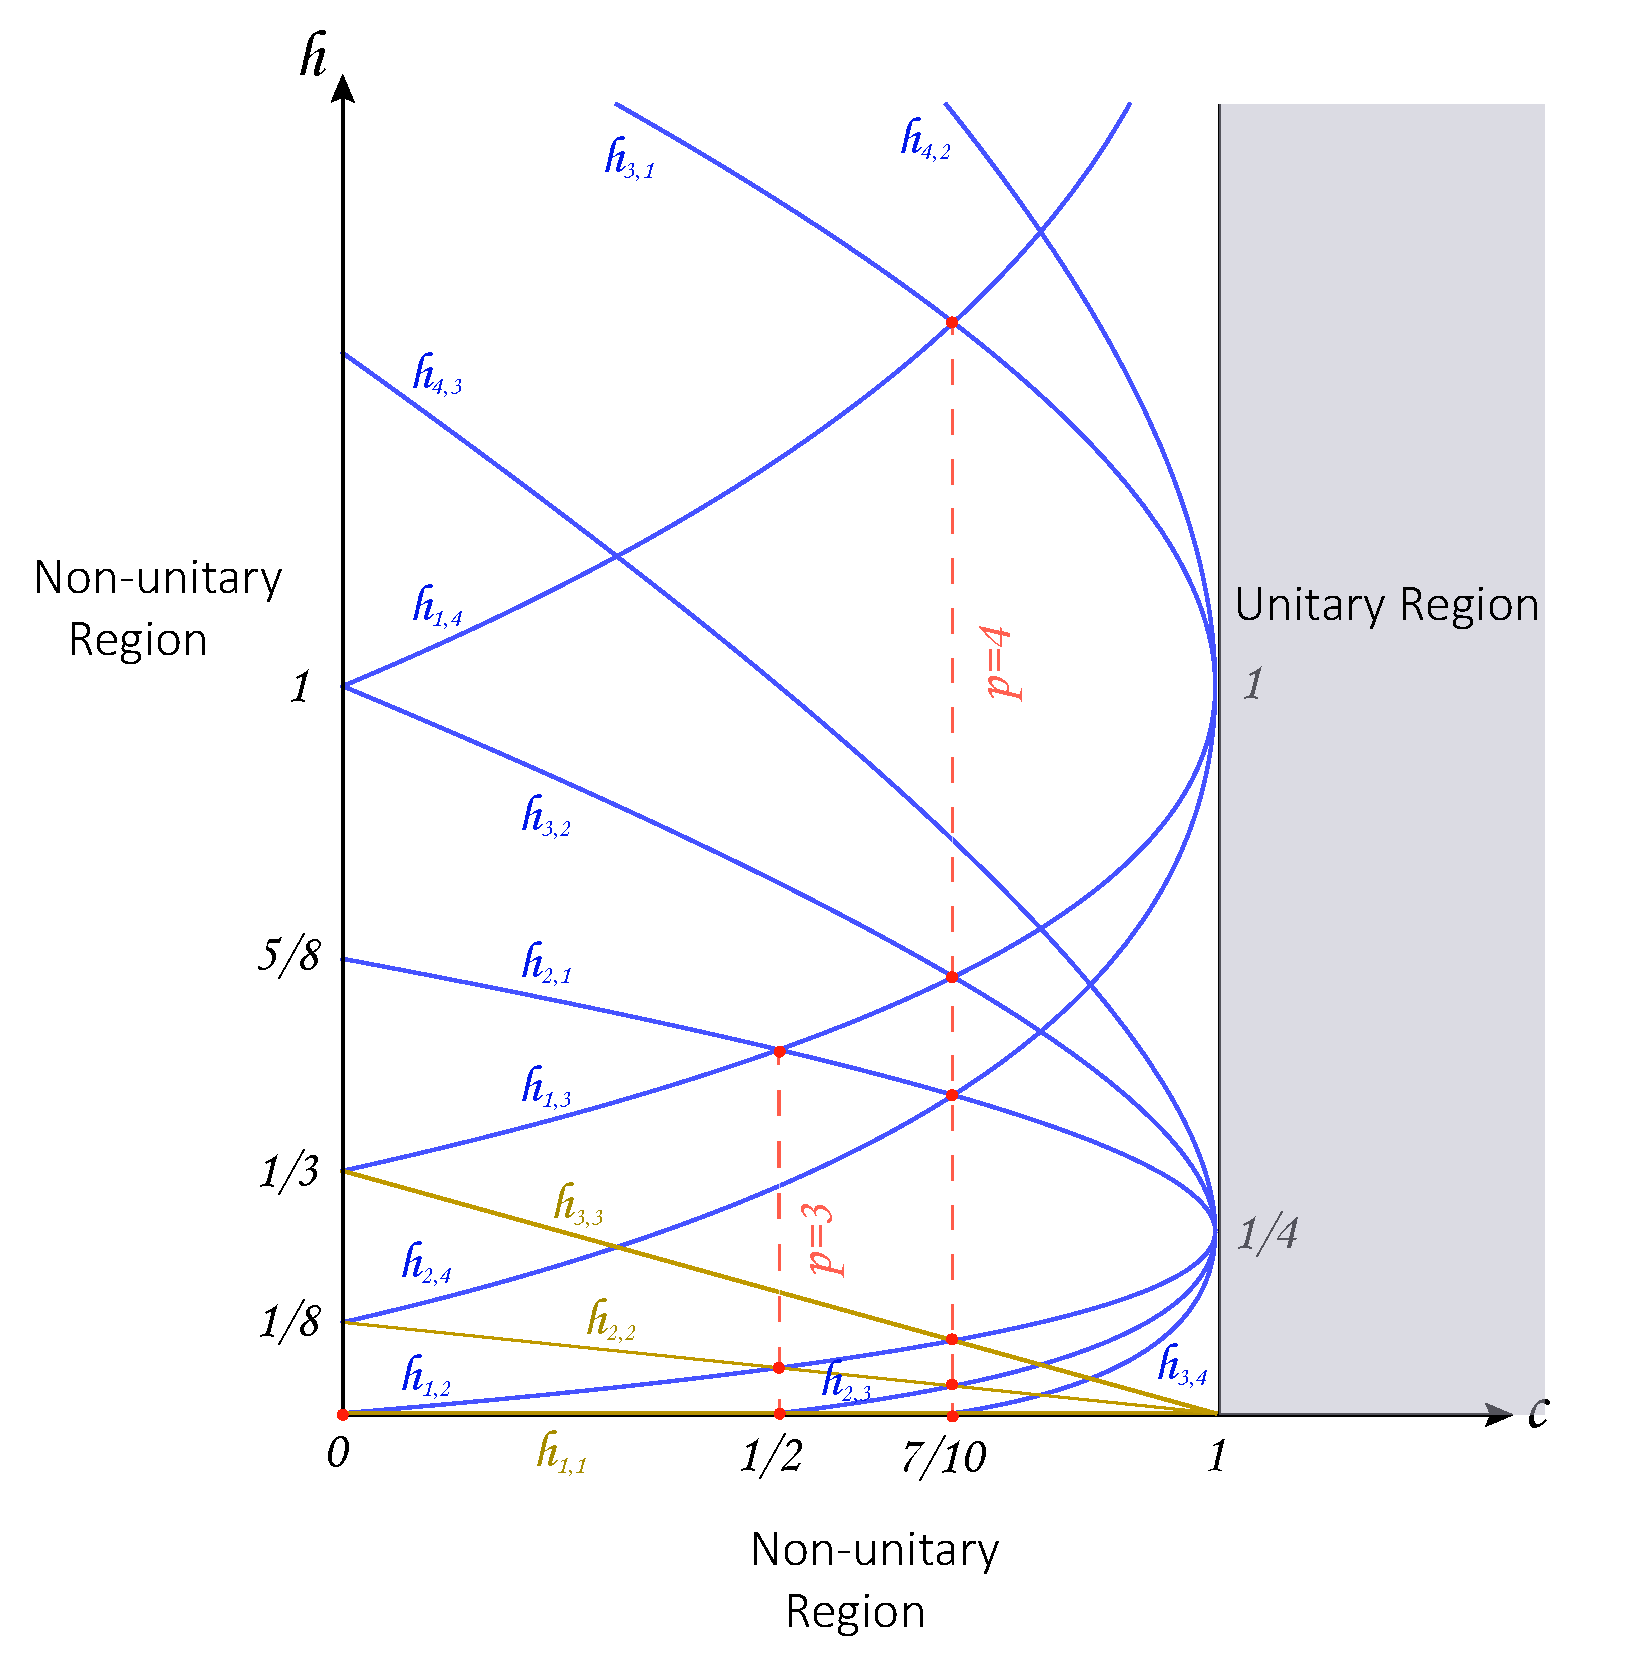
\includegraphics[width=.8\linewidth]{picture/Kac-Determinant}
	\caption{Kac determinant}
	\label{fig:kac-determinant}
\end{figure}

Kac has found a closed form expression of the determinant of $N$ level Gram matrix, which is called \textbf{Kac determinant}  \cite[ISZ88-No.7]{kac1979contravariant}
\begin{equation}
\label{Kac-determinant}
\operatorname{det } M _{N } (c , h)=\alpha _{N } \prod _{r,s  \leq N } \left(h-h _{r,s } (c) \right)^{P (N-rs) }\, ,
\end{equation}
where $\alpha_N$ is a positive constant independent of $c$
and $h$. The Kac determinant provides the complete information of null states in a Verma module.
From this expression, one can see that a null state first appears at level $n=rs$ if $h=h_{r,s}$. Thus at level $N>rs$, the
zero order for $h_{r,s}$ is $P(N-rs)$. In fact, there are two useful equivalent way to write $h_{r,s}$; the first expression is
\bea
\label{rel-hrs-alpha}
 h _{r,s } (c) &= h _{0 } + \frac{1 }{4 } \left(r \alpha _{+ } + s \alpha _{- } \right)^{2 }\, ,\notag\\
 h _{0 } &= \frac{1 }{24 } (c-1)\, ,\\
 \alpha _{\pm } &= \frac{\sqrt{1-c } \pm \sqrt{25-c } }{\sqrt{24 } }\, ,\notag
\eea
and the second is
\bea
\label{rel-hrs-m}
h _{r,s } (p) &= \frac{[ (p + 1) r-p s ]^{2 }-1 }{4 p (p + 1) }\, ,\notag\\
c &= 1-\frac{6 }{p (p + 1) }\, ,
\eea
where $m$ has two branches
\begin{equation}
\label{m branches}
p=- \frac{1 }{2 } \pm \frac{1 }{2 } \sqrt{\frac{25-c }{1-c } }
\end{equation}
From this expression, one can see that when $c=1$, a Verma module is irreducible if $h\neq n^2/4$ for $n\in\bZ$. In addition, when $c=0$, a Verma module is irreducible if $h\neq (n^2-1)/24$ for $n\in\bZ$.

Both of the above expression provide the following
result for $h_{r,s}(c)$, which is illustrated  in Figure \ref{fig:kac-determinant}
\begin{equation}
\label{rel-hrs}
  h _{r,s } (c)=\frac{1-c }{96 } \left[ \left((r + s) \pm (r-s) \sqrt{\frac{25-c }{1-c } } \right)^{2 }-4 \right]\, .
\end{equation}
One can convince oneself that $h_{1,2}$ and $h_{2,1}$ are as in \eqref{level-2}.
The Kac determinant changes sign when the values of $(c,h^2)$ cross
each curve $h=h_{r,s}(c)$.



\subsubsection*{Minimal models $\cM_{p,p'}$}
Belavin-Polyakov-Zamolodchikov have noticed that all the correlation functions can be determined by differential equations when the Kac determinant becomes zero.
As an example, let us first consider the situation in which there are null states at the level two. In general, a null state $\ket{\chi}$ at level two takes the form \begin{equation}
\ket{\chi}=L _{- 2 } | h \rangle + a L _{- 1 }^{2 } | h \rangle \, .
\end{equation}
By applying the $L_1$ to the above equation, we have
\bea
\left[ L _{1 } , L _{- 2 } \right] | h \rangle + a \left[ L _{1 } , L _{- 1 }^{2 } \right] | h \rangle &= 3 L _{- 1 } | h \rangle + a \left(L _{- 1 } 2 L _{0 } + 2 L _{0 } L _{- 1 } \right) | h \rangle\notag \\
&= (3 + 2 a (2 h + 1)) L _{- 1 } | h \rangle=0
\, ,
\eea
which requires that
\begin{equation}
a=- 3 / 2 (2 h + 1)\, .
\end{equation}
By applying $L_2$, we find that
\bea
\left[ L _{2 } , L _{- 2 } \right] | h \rangle + a \left[ L _{2 } , L _{- 1 }^{2 } \right] | h \rangle &= \left(4 L _{0 } + \frac{c }{2}\right) | h \rangle + 3 a L _{1 } L _{- 1 } | h \rangle \notag \\
&= (4 h + c / 2 + 6 a h) | h \rangle=0\, .
\eea
Therefore the central charge must satisfy
\begin{equation}
c=2(-6ah-4h)=2h\frac{5-8h}{2h+1}
\end{equation}
Writing $h$ in terms of $c$, we have
\begin{equation}
h=\frac{1}{16}\left\{
5-c\pm \sqrt{(c-1)(c-25)}
\right\}\, ,
\end{equation}
which are equal to $h_{1,2}$ and $h_{2,1}$ in \eqref{level-2}.




Since the null state $\ket{\chi}$ is orthogonal to any states in the Verma module, we have
$$
 \langle \chi (z) X \rangle =0
$$ where $X$ is a product of any primary fields as usual.
By using
\eqref{differential-equation}, the correlation function
$\expval{\phi(z)X}$ should be governed by the
following differential equation
\begin{equation}
\left\{\mathcal{L } _{- 2 }-\frac{3 }{2 (2 h + 1) } \mathcal{L } _{- 1 }^{2 } \right\} \langle \phi (z) X \rangle=0\, ,
\end{equation}
where  $\phi(z)$ has conformal dimension $h_{1,2}$ or
$h_{2,1}$.
One can write the above expression as a differential equation
\begin{equation}
\left\{\sum _{i=1 }^{N } \left[ \frac{1 }{z-z _{i } } \frac{\partial }{\partial z _{i } } + \frac{h _{i } }{\left(z-z _{i } \right)^{2 } } \right]-\frac{3 }{2 (2 h + 1) } \frac{\partial^{2 } }{\partial z^{2 } } \right\} \langle \phi (z) X \rangle=0\, .
\end{equation}
If $X$ is $\phi(w)$ itself, the differential
equation for two point function becomes
\begin{equation}
\left\{\frac{1 }{z-w } \partial _{w } + \frac{h }{(z-w)^{2 } }-\frac{3 }{2 (2 h + 1) } \partial _{z }^{2 } \right\} \langle \phi (z) \phi (w) \rangle=0\, ,
\end{equation}
which is satisfied by the general form for
two-point function $\expval{\phi(z)\phi(w)}=(z-w)^{-2h}$.
For three point function, $X=\phi_1(z_1)
\phi_2(z_2)$, we have
\begin{equation}
\left\langle \phi (z) \phi _{1 } \left(z _{1 } \right) \phi _{2 } \left(z _{2 } \right) \right\rangle=\frac{C_{h,h_1,h_2} }{\left(z-z _{1 } \right)^{h _{2 }-h-h _{1 } } \left(z _{1 }-z _{2 } \right)^{h-h _{1 }-h _{2 } } \left(z-z _{2 } \right)^{h _{1 }-h-h _{2 } } }\, .
\end{equation}
The differential equation gives further constraint to
the highest weights of field operators in the three-point function.
\begin{equation}
h _{2 }=\frac{1 }{6 } + \frac{1 }{3 } h + h _{1 } \pm \frac{2 }{3 } \sqrt{h^{2 } + 3 h h _{1 }-\frac{1 }{2 } h + \frac{3 }{2 } h _{1 } + \frac{1 }{16 } }\, .
\end{equation}
For $h=h_{1,2}$, and set $h_1=h_{r,s}$ in
\eqref{rel-hrs}, we find $h_2$ equals to $h_{r,s-1}$
or $h_{r,s+1}$. Similarly for $h=h_{2,1}$, we have
$h_2$ equals to $h_{r-1,s}$ or $h_{r+1,s}$. Recall that
the two point function has non-vanishing value only
when the two field operators within it has the same highest weight. We thus have the following operator algebra
\bea
\phi _{1,2} \times \phi _{r,s} &=[ \phi _{r,s-1} ]+ [\phi _{r,s + 1}]\notag \\
\phi _{2,1} \times \phi _{r,s} &= [\phi _{r-1 , s}] + [\phi _{r + 1 ,s}]\, ,
\eea
where $\phi_{r,s}$ means the field operator with highest
weight $h_{r,s}$. The expression above means that the
fields $\phi _{1,2}$ and $\phi_{2,1}$ act as
ladder operators in the operator algebra. In addition,
the field operators expanded in the right side not only
contain the primary fields but their descendant fields
as well. The coefficient on the right side may be zero.
For instance,
\bea
\phi _{1,2} \times \phi _{2,1} &=[ \phi _{2,0} ]+ [\phi _{2,2}]\, ,\notag \\
\phi _{2,1} \times \phi _{1,2} &= [\phi _{0,2}] + [\phi _{2,2}]\, .
\eea
Since the two OPEs are equivalent, this shows the coefficients before $\phi _{2,0}$ and
$\phi _{0,2}$ must be zero.
Therefore, we have
\begin{equation}
\phi _{1,2} \times \phi _{2,1} =[ \phi _{2,2}]\, .
\end{equation}
The above expression can be generalized to
the following fusion rules
\begin{equation}
\label{fusion-rule-1}
\phi_{r_1, s_1}\times \phi_{r_2,s_2}
= \sum_{
	\begin{subarray}{1}
	\quad k=1+\abs{r_1-r_2}\\
	k+r_1+r_2=1\,\text{mod}\, 2
	\end{subarray}
  }^{k= r_1 + r_2 -1}
\,
\sum_{
	\begin{subarray}{1}
	\quad l=1+\abs{s_1-s_2}\\
	l+s_1+s_2=1\,\text{mod}\, 2
	\end{subarray}
}^{l= s_1 + s_2 -1}
[\phi_{k,l}]\, .
\end{equation}
The summation variables $k$ and $l$ are incremented
by $2$. The expression above implies that
the conformal family $[\phi_{r,s}]$ forms a
closed operator algebra.
\begin{figure}
	\centering
	\includegraphics[width=0.6\linewidth]{picture/minimal-model}
	\caption{"diagram of dimensions"}
	\label{fig:minimal-model}
\end{figure}









The  operator algebra
\eqref{fusion-rule-1}, implies there are infinite
number of conformal families present in the theory.
However, we want a finite set of highest weight in
a minimal model. In order to understand the situation
graphically, we consider the "diagram of dimensions" as in Figure
\ref{fig:minimal-model}.
The points $(r,s)$ in the first quadrant label the various conformal dimensions appearing in the Kac formula.
The dotted line has a slope $\tan\theta=-\alpha_+/\alpha_-$, where $\alpha_{\pm }$ are defined
in \eqref{rel-hrs-alpha}. If $\delta$ is the distance
between a point $(r,s)$ and the dotted line. It is
a good exercise to show the following relation,
\begin{equation}
h _{r , s }=h _{0 } + \frac{1 }{4 } \delta^{2 } \left(\alpha _{+ }^{2 } + \alpha _{- }^{2 } \right)\, .
\end{equation}
If the slope $\tan\theta$ is irrational, it will never
go through any integer point $(r,s)$, which means
$\delta$ is always non-zero. There is no periodical
property for $h_{r,s}$. However, if the slope
$\tan \theta$ is rational. That is, if there exist
two coprime integers $p$ and $p'$ such that
\begin{equation}
p^{\prime } \alpha _{- } + p \alpha _{+ }=0\, .
\end{equation}
The dotted line will go through the point $(p',p)$, we
have the following periodicity property.
\begin{equation}
h _{r, s }=h _{r + p, s + p^{\prime }}\, .
\end{equation}
Therefore, there are finitely many primary fields and we call it the \textbf{minimal model} denoted by $\cM_{p,p'}$.
Using \eqref{rel-hrs-alpha}, the central charge and
the Kac formula become
\bea
\label{minimal_model}
c &= 1-6 \frac{\left(p-p^{\prime } \right)^{2 } }{p p^{\prime } }\notag \, ,\\
h _{r , s } &= \frac{\left(p^{\prime } r-p s \right)^{2 }-\left(p-p^{\prime } \right)^{2 } }{4 p p^{\prime } }\, .
\eea
We can obtain a symmetry property from above:
\begin{equation}\label{inversion-formula}
h _{r , s  }=h _{p -r, p^{\prime }-s }\, .
\end{equation}
Now, we get a finite set of conformal families, which
closes under fusion rules. The corresponding finite
set of conformal dimensions $h_{r,s}$ is given by
$1\leq r < p$ and $1 \leq s < p^{\prime }$, and thus
construct a minimal model. The symmetry above
gives
\begin{equation}
\phi _{r , s }=\phi _{p-r , p^{\prime }-s  }\, .
\end{equation}
Hence, there remain $(p-1)(p'-1)/2$ distinct fields in the
theory.
And the fusion rule is modified to be
\begin{equation}\label{MM-fusion}
\phi _{r,s}\times\phi _{m,n}=
\sum^{k_{\text{max}}}_{
\begin{subarray}{1}
  \quad  k=1+ \abs{r-m} \\
  k+r+m=1 \, \text{mod} \, 2
\end{subarray}}
\,
\sum^{l_{\text{max}}}_{
	\begin{subarray}{1}
	\quad  l=1+ \abs{s-n} \\
	k+s+n=1 \, \text{mod} \, 2
	\end{subarray}}
\left[\phi _{k,l}\right]\, ,
\end{equation}
where the upper bound of the summation now is control
by the periodical and symmetric condition.
\bea
k _{\max } &= \min \left(r + m-1,2 p -1-r-m \right)\, ,\\
l _{\max } &= \min (s + n-1,2 p^{\prime }-1-s-n)\, .
\eea
We will see several examples of minimal models in the following subsections.





























\subsubsection*{Unitarity for $c> 1$}


We can further use Kac determinant to derive unitarity condition.
In fact, the unitary condition gives us great constraint of
the choice of $h$ and $c$, especially in the
region $0\le c\le1$.









The explicit expression for the Kac determinant allow
us to prove the representations $(c>1,h>0)$ are unitary. The proof is down by three steps:

The first step is to show the curves $C_{r,s}: h= h_{r,s}$ lie
below or on the axis $h=0$ if $c>1$.
if $1<c<25$, from \eqref{rel-hrs}, we see that $h_{r,s}$ is not
a real number unless $s=r$, in which $h_{r,s}\leq0$.
On the other hand, if $c\geq 25$ the choice
\eqref{m branches} implies that $-1<m<0$.
Then $p(p+1)<0$ and
$[(p+1)r-ps]\geq 1$ which implies $h_{r,s}(p)\leq0$
according to \eqref{rel-hrs-m}. Thus we have shown that
all the curves $C_{r,s}$ are located below the
$h=0$ axis if $c>1$.

The second the step is to prove that the Kac determinant is positive throughout the region.
For a given level, we can find a $h$ larger than
any $h_{r,s}$, and at such a point Kac determinant is
positive. Since none of the curves lies in the
region, the determinant sign can not be changed through out the region by crossing any curves.
This proves the second point.

The last step is to prove that the
Gram matrix at level $N$, $M_N$ is positive definite in
this region, which is equivalent to the theory
in this region is unitary.
Since the Kac determinant is positive, the
number of negative eigenvalues of $M_N$ must be
even. Since the number can change only across one
of the curves $C_{r,s}$, and consequently must stay
the same throughout the region. Therefore, we just need
to show that the matrix $M_N$ for each level $N$ is positive definite for at least one point $(c,h)$.

In order to do this, we define the length $n(\alpha)$
of a basis vector $\ket{\alpha}$ as the number of
operators $L_k$ used to define it. For instance,
$L^{3}_{-1}$ has length $3$ and $L_{-3}\ket{h}$ has
length 1.
It is possible to show that the dominant behavior
in $h$ of inner products is
\bea
  \langle \alpha | \alpha \rangle &= c _{\alpha } h^{n (\alpha) } [ 1 + O (1 / h) ] \quad \left(c _{\alpha } > 0 \right)\\
  \langle \alpha | \beta \rangle &= O \left(h^{(n (\alpha) + n (\beta)) / 2-1 } \right) + \ldots
  \, .
\eea
where $\ket{\alpha}$ and $\ket{\beta}$. The above
expression immediately shows that $M_N$ is dominant by
its diagonal element when $h$ is sufficiently
large, and thus $M_N$ is positive definite. Therefore, in this region, a Verma module $V(c,h)$ is irreducible.

\subsubsection*{Unitarity for $0 \le c \le 1$}
In this region, we just roughly gives some statements.
First, it is easy to show that, in Figure \ref{fig:kac-determinant}, one may
connect any point in the region $0\le c\le1$, $h>0$ to the $c>1$ region by a path that crosses a single
vanishing curve of the Kac determinant at some level.
The determinant reverses sign when passing through
the vanishing curve. Therefore, there must be a
negative norm state at that level. This excludes
unitary representations of the Virasoro algebra at
all points in this region, except those on the vanishing curves themselves.
A more careful analysis shows that there is
an additional negative norm state everywhere on
the vanishing curves except at certain points
where they intersect.

Therefore, the unitary representations of the
Virasoro algebra only occur at the values of
the central charge \cite[ISZ88-No.3]{Cardy:1984bb}:
\begin{equation}
\label{c<1-unitary-c}
c=1-\frac{6 }{p (p + 1) } \, ,\quad p=3,4 , \ldots
\end{equation}
with corresponding highest weight
\begin{equation}
\label{c<1-unitary-hrs}
h _{r,s } (p)=\frac{[ (p + 1) r-p s ]^{2 }-1 }{4 p (p + 1) }\, .
\end{equation}
where $r,s$ satisfies $1 \leq s \leq r \leq p-1$. The form is exactly the same as \eqref{rel-hrs-m}, but now $p$ can only take discrete
integers. This result tells us that the unitary
condition is satisfied only at the point $(h,c)$ where
the Verma module has null states.

\subsubsection*{Unitary Minimal Models $\cM_p$}
We now consider the choice of $p$ and $p'$ to make
the minimal models unitary. Recalling the
admissible conformal dimensions in \eqref{minimal_model},
Bezout's lemma states that there exists a couple
of integers $(r_0,s_0)$ in the range $1\leq r_0 < p$ and $1 \leq s_0 < p^{\prime }$ such that
\begin{equation}
p^{\prime } r _{0 }-p  s _{0 }=1\, .
\end{equation}
Thus, the corresponding conformal dimension
\begin{equation}
h _{r _{0 } , s _{0 } }=\frac{1-\left(p-p^{\prime } \right)^{2 } }{4 p p^{\prime } }
\, ,
\end{equation}
which is always negative, expect if
$\abs{p-p'} =1$, in which case it vanishes. In fact, the minimal model is unitary only if $\abs{p-p'} =1$, and the primary field $h _{r _{0 } , s _{0 } } =0$ is indeed the identity operator.
Hence, we can set $p'=p+1$ so that the central charge is expressed in \eqref{c<1-unitary-c}. We denote the unitary minimal model by $\cM_p$.
We note that the list of unitary representations given in \eqref{c<1-unitary-c} and
\eqref{c<1-unitary-hrs}, coincides with the list
of highest weight $h_{r,s}$ of unitary minimal models.




\subsection{Characters of minimal models }\label{sec:characters-MM}
The character of an irreducible representation of the Virasoro algebra
$$
\chi _{h } (\tau) \equiv \operatorname{Tr } _{L(c,h) } q^{L _{0 } -\frac{c}{24} }=q^{-\frac{c}{24} } \sum _{N=0 }^{\infty } d _{h } (N) q^{h + N }~,
$$
where $d_h(N)$ is the number of states at level $N$, and $d_h(N)\le P(N)$. If there is no null state, $d_h(N)=P(N)$.
Th partition function with periodic boundary conditions on a torus is
\bea
Z _{\mathrm{PP } } (\tau , \overline{\tau }) &= \operatorname{Tr } \left(q^{L _{0 }-c / 24 } \overline{q }^{\overline{L } _{0 }-c / 24 } \right)\cr
&= \sum _{h , \overline{h} } \mathcal{N } _{h \overline{h } } ~\chi _{h } (\tau) \chi _{\overline{h}} (\overline{\tau })~,
\eea
where $ \mathcal{N } _{h \overline{h } } $ is the number of primary fields of conformal dimension $(h,\overline h)$ \cite[ISZ88-No.25]{cardy1986operator}. Since there is only one vacuum, we set $\cN_{00}=1$. Under the $T$-transformation, a character behaves as
\be\label{T-trans}
\chi _{h } (\tau + 1)=e^{2 \pi i (h-c / 24) } \chi _{h } (\tau)~.
\ee
The invariance of $\cZ_{\mathrm{PP}}$ under the $T$-transformation requires
$$\mathcal{N } _{h \overline{h} }=0 , \quad h-\overline{h } \notin \mathbb{Z }~.$$
If we write the $S$-transformation of characters
$$\chi _{h } (-1/\tau)=\sum _{h^{\prime } } S _{h h^{\prime } } ~\chi _{h^{\prime } } \left(\tau \right)~,$$
then the modular invariance of $\cZ_{\mathrm{PP}}$ requires
\begin{equation}
\label{relation N S}
\sum _{h , \overline{h} } \mathcal{N } _{h \overline h } S _{h h' } S _{\overline{h } \overline{h}^{\prime } }=\mathcal{N } _{h^{\prime } \overline{h}^{\prime } }~.
\end{equation}
Below we will determine the partition function of diagonal type $\cN_{hh'}=\delta_{hh'}$ in the unitary minimal models.. We will see one example of non-diagonal type in the tricritical Ising model in \S\ref{sec:examples}, and the classification of the modular invariant partition functions are discussed in the end of \S\ref{sec:su2k-character}.

From the Kac determinant, we have learnt that the Verma module $V_{h_{r,s}}$ has a singular vector at level $rs$. Since $h_{r,s}+rs=h_{-r,s}$, the singular vector generates a submodule $V_{h_{-r,s}}$. Furthermore. since $h_{p-r,p'-s}+ (p-r) (p'-s)=h_{2p-r,s}$, we have another submodule $V_{h_{2p-r,s}}$. Moreover, these submodule $V_{h_{-r,s}}$, $V_{h_{2p-r,s}}$ contain other submodules $V_{h_{-2p-r,s}}$, $V_{h_{2p+r,s}}$, and one can see repeatedly this pattern \cite[ISZ88-No.9]{feigin1983verma}.


\begin{figure}[ht]
\centering
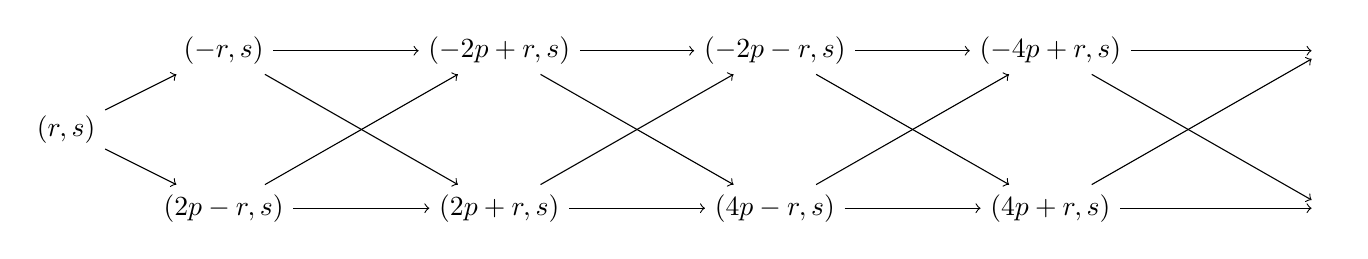
\begin{tikzpicture}[node distance=3.5cm]
\node (A) at (0,0){$(r,s)$};
\node (B) at (2,1){$(-r,s)$};
\node (C) at (2,-1){$(2p-r,s)$};
\node [ right of =B] (D){$(-2p+r,s)$};
\node [ right of =D] (E){$(-2p-r,s)$};
\node [ right of =E] (F){$(-4p+r,s)$};
\node [ right of =F] (F1){$\ $};
\node [ right of =C] (G){$(2p+r,s)$};
\node [ right of =G] (H){$(4p-r,s)$};
\node [ right of =H] (I){$(4p+r,s)$};
\node [ right of =I] (I1){$\ $};
\draw[->] (A) -- (B);
\draw[->] (A) -- (C);
\draw[->] (B) -- (D);
\draw[->] (D) -- (E);
\draw[->] (E) -- (F);
\draw[->] (C) -- (G);
\draw[->] (G) -- (H);
\draw[->] (H) -- (I);
\draw[->] (F) -- (F1);
\draw[->] (I) -- (I1);
\draw[->] (B) -- (G);
\draw[->] (D) -- (H);
\draw[->] (E) -- (I);
\draw[->] (C) -- (D);
\draw[->] (G) -- (E);
\draw[->] (H) -- (F);
\draw[->] (F) -- (I1);
\draw[->] (I) -- (F1);
\end{tikzpicture}
\end{figure}



Therefore, the character of the irreducible representation $L(c,h_{r,s})$ of the Virasoro algebra is
$$
\begin{aligned} \chi _{r, s } (\tau) &=\operatorname{Tr } _{L(c,h_{r,s}) } q^{L _{0 } -\frac{c}{24} } \\ &=\frac{1 }{q^{-1/24}\eta (\tau) } q^{-\frac{c}{24} } \sum _{k \in \mathbb{Z } }\left[ q^{h _{r + 2 p k , s } }-q^{h _{2 p k-r  },  s } \right] \end{aligned}$$
which is called the \textbf{Rocha-Caridi formula} \cite[ISZ88-No.10]{rocha1985vacuum}.

Defining the theta functions by
\begin{equation}
\label{Theta function}
\Theta _{m , k } (\tau)=\sum _{n \in \mathbb{Z } } q^{k \left(n + \frac{m }{2 k } \right)^{2 } }
\end{equation}
it can be written by
\be\label{Rocha-Caridi-formula}
\chi _{r, s } (\tau)=\frac{1 }{\eta (\tau) } \left(\Theta _{r (p + 1)-s p , p (p + 1) } (\tau)-\Theta _{r (p + 1) + s p , p (p + 1) } (\tau) \right)
\ee
The behavior of $\chi_{r,s}(\tau)$ under the $S$-transformation has been obtained in  \cite[ISZ88-No.29]{Cardy:1986gw}:
\bea\label{RC-S}
 \chi _{r, s } (- 1 / \tau)&= \sum _{1 \leqq s^{\prime } \leqq r^{\prime } \leq p-1 }S_{(r,s),(r',s')} ~\chi _{r^{\prime } s^{\prime } } (\tau) \cr
S_{(r,s),(r',s')} &=\left(\frac{8 }{p (p + 1) } \right)^{1 / 2 } (- 1)^{(r + s) \left(r^{\prime } + s^{\prime } \right) } \sin\left( \frac{\pi r r^{\prime } }{p } \right)\sin \left(\frac{\pi ss^{\prime } }{p + 1 }\right)
\eea
and the $T$-transformation is given in \eqref{T-trans}.
It is shown that the partition function of diagonal type
\be\label{diagonal-PP}
\cZ_{\cM_p}^{\textrm{diag}}=\sum _{1 \leqq r \leqq s \leq p-1 } \left| \chi _{r, s } (\tau) \right|^{2 }
\ee
is invariant under the modular transformations.




\subsection{Ising model $(p',p)=(4,3)$}\label{sec:Ising}
\begin{table}[htbp]\centering
\begin{tabular}{c|cc}
		$3$
		& $\frac{1}{2}$
		& $0$
		\\[5pt]
				$2$
		& $\frac{1}{16}$
		& $\frac{1}{16}$
		\\[5pt]
		$1$
		& $0$
		& $\frac{1}{2}$
		\\[5pt]
		\midrule
		& $1$
		& $2$
	\end{tabular}
	\hspace{2cm}
	\begin{tabular}{c|cc}
		$3$
		& $\varepsilon$
		& $\mathbf{1}$
		\\[5pt]
				$2$
		& $\sigma$
		& $\sigma$
		\\[5pt]
		$1$
		& $\mathbf{1}$
		& $\varepsilon$
		\\[5pt]
		\midrule
		& $1$
		& $2$
	\end{tabular}\end{table}
Let us consider the unitary minimal  model $\cM_{p=3}$ whose the central charge $c=\frac12$. The primary fields and their conformal dimensions  are described in the table above. By comparing the conformal dimensions with \eqref{Ising-conf-dim}, $\varepsilon$ is the energy density operator and $\sigma$ is the spin field in the Ising model. Therefore,   the unitary minimal  model $\cM_{p=3}$ describes the Ising model.




Since the Ising model is the most important 2d CFT, let us investigate it more in detail. For the Ising model on a lattice of $(N\times M)$ sites, the statistical partition function is
$$
\cZ=\sum_{\{\sigma\}}e^{-K\sum_{ij}\sigma_i\sigma_j}
$$
where we define $K=J/(k_BT)$. One can use the identity
$$
\exp \left[ x \sigma _{i } \sigma _{l } \right]=\cosh x \left(1 + \sigma _{i } \sigma _{l } \tanh x \right)
$$
so that the partition function is
$$
\cZ=\sum _{\{\sigma \} } \prod _{\{i j \} } \cosh (K) \left(1 + \sigma _{i } \sigma _{j } \tanh (K) \right)~.
$$
At high-temperature, $\tanh K$ is small and one can take expansion. In the expansion, the generic expression of these terms is
$$
\tanh(K)^{r } \sigma _{1 }^{n _{1 } } \sigma _{2 }^{n _{2 } } \sigma _{3 }^{n _{3 } } \ldots
$$
where $r$ is the total number of  lines connecting the adjacent sites $i$ and $j$, and $n_i$ is the number of lines where $i$ is the final site. Since each spin $\sigma_i$ assumes values $\pm1$, we have a null sum unless all $n_1, n_2, \ldots$ are even numbers, which implies all closed loops $P$ of the lattice as in Figure \ref{fig:high-temp}. Hence, the partition function is
$$
\cZ _{\mathrm{high } }=[ 2 \cosh (K) ]^{N M } \sum _{P } [ \tanh (K) ]^{\mathrm{lengh } (P)}
$$
\begin{figure}[ht]\centering
\includegraphics[width=4cm]{picture/lattice1}\hspace{2cm}\includegraphics[width=4cm]{picture/lattice2}\label{fig:high-temp}
\end{figure}




On the other hand, at low temperature, the spins tend to align one with another. Taking the dual lattice, the boader  between antiparallel spins form loops $P_D$, and the partition function is given by
$$
\cZ _{\mathrm{low } }=2 e^{N M K } \sum _{P_D } e^{- 2 K (\mathrm{length }(P_D)) }~.
$$
where the contribution of all spins down has been factored out of the sum.






\begin{figure}[ht]\centering
\includegraphics[width=5cm]{picture/lattice3}\hspace{2cm}\includegraphics[width=5cm]{picture/lattice4}
\end{figure}



The two phases are indeed dual to each other
$$
\cZ _{\mathrm{low } } \left(K^{\prime } \right)=2 (\sinh 2 \mathrm{K })^{- N M / 2 } \cZ _{\mathrm{high } } (K)
$$
where we identify
$$
e^{- 2 K^{\prime } }=\tanh K~.
$$
This is called the \textbf{Kramers-Wannier duality}.

Let us recall the Hamiltonian \eqref{Ising-Hamiltonian} of the Ising model
\be\label{Ising-Hamiltonian2} \mathcal{H}=- J \sum _{\left\langle i , i^{\prime} \right\rangle} \sigma _{i}^z \sigma _{i^{\prime}}^z-B \sum _{i} \sigma _{i}^x
\ee
Here we assume that the external magnetic field $B$ is parallel to the $x$-axis. In the low-temperature $J\gg B$, we can ignore the interaction with the external magnetic field $B$. However, in the high-temperature $J\ll B$, this is not the case. In order to capture the interaction term,  it is natural to consider the \textbf{disorder operator} $\mu_i$ on the dual lattice, which is defined as follows:
$$\mu _{a }^{z } \equiv \prod _{i=- N / 2 }^{i=a } \sigma _{i}^{x }~,\qquad
\mu _{a }^{x }=\sigma _{a }^{z } \sigma _{a + 1 }^{z }
$$
For instance, if we act  $\mu^z_a$ on the parallel-spin state
$$
| \uparrow \rangle \equiv \prod _{b=- N / 2 }^{N / 2 } | \uparrow \rangle _{b }
$$
then we have
$$
\mu _{a }^{z } | \uparrow \rangle=\prod _{b=- N / 2 }^{a } | \downarrow \rangle _{b } \prod _{c=a + 1 }^{N / 2 } | \uparrow \rangle _{c }
$$
Thus, the disorder operator $\mu _{a }^{z }$ changes the ordered spin configurations at the dual site $a$ so that it can be understood as a \textbf{soliton} located at the dual site $a$.  Moreover, the Hamiltonian \eqref{Ising-Hamiltonian2} can be written as
$$
 \mathcal{H}=- B \sum _{\left\langle a,a^{\prime} \right\rangle} \mu _{a}^z \mu _{a^{\prime}}^z-J \sum _{a} \mu _{a}^x
$$
so that $B$ and $J$ are exchanged. Hence, in the low-temperature
$$
\left\langle \sigma _{a }^{z } \right\rangle \neq 0 , \quad \left\langle \mu _{a }^{z } \right\rangle=0 , \quad T < T _{c }
$$
whereas in the high-temperature
$$
\left\langle \mu _{a }^{z } \right\rangle \neq 0 , \quad \left\langle \sigma _{a }^{z } \right\rangle=0 , \quad T > T _{c }~.
$$
Thus, the Kramers-Wannier duality  exchanges the spin and disorder operator $\sigma\leftrightarrow\mu$. Hence, $\sigma$ and $\mu$ have the same conformal dimension. In fact, they are called \textbf{mutually non-local}, meaning that one obtains the minus sign
$$
\sigma (z , \overline{z }) \mu (0,0) \rightarrow \sigma \left(e^{2 \pi i } z , e^{- 2 \pi i  }\overline{z } \right) \mu (0,0)=- \sigma (z , \overline{z }) \mu (0,0)
$$
when $\sigma$ is rotated around $\mu$. From this fact, the fermion shows up in the OPE of $\sigma$ and $\mu$
\be\label{sigma-mu}
\sigma (z , \overline{z }) \mu (0,0)\sim\frac{1 }{| z |^{\frac14} } \left(z^{1 / 2 } \psi (0) + \overline{z }^{1 / 2 } \overline{\psi } (0) \right)
\ee
Recalling that the central charge of the minimal model $\cM_{p=3}$ is $c=\frac12$, one can deduce that the continuum limit of the Ising model is described by a free fermion.

\begin{figure}[ht]\centering
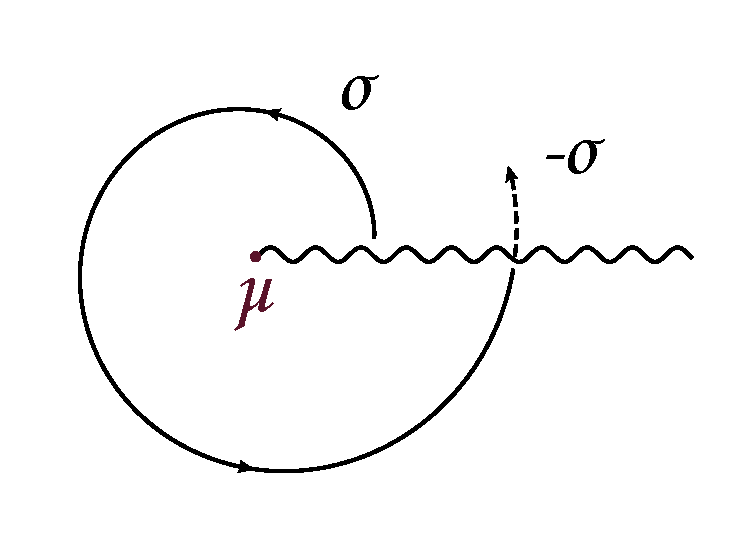
\includegraphics[width=6cm]{picture/order-disorder}
\end{figure}

In fact, the various operators are identified  as
\bea
\psi (z)& \sim\phi _{2,1 } (z) \otimes \phi _{1,1 } (\wt{z }) \cr \overline{\psi } (\overline{z })& \sim\phi _{1,1 } (z) \otimes \phi _{2,1 } (\overline{z }) \cr
\psi \overline{\psi } : =\varepsilon (z , \overline{z })&\sim \phi _{2,1 } (z) \otimes \phi _{2,1 } (\overline{z })\cr
 \sigma (z , \overline{z }) \ \textrm{or} \ \mu (z , \overline{z }) &\sim\phi _{1,2 } (z) \otimes \phi _{1,2 } (\overline{z })
 \eea
 and the operator algebras are read off
$$
\sigma \cdot \sigma=\mathbf{1 } + \varepsilon ~,\qquad  \varepsilon \cdot \varepsilon=\mathbf{1 } ~,\qquad  \sigma \cdot \varepsilon=\sigma~.
$$

Moreover, using the associativity of OPEs, one can derive from \eqref{sigma-mu}
$$
\psi ( z ) \sigma ( w,\overline w ) \sim \frac{1}{( z - w ) ^ { 1 / 2}} \mu ( w ,\overline w)~.
$$
W can compare this with the mode expansion of free fermion on the Ramond sector
$$\psi ( z ) \sigma ( 0 ) = \sum _ { r \in \bZ} z ^ { - r - 1 / 2 } b _ { r } \sigma ( 0 )~,$$
we can deduce
$$b _ { 0 } \sigma ( 0 ) = \mu ( 0 )~.$$
In the presence of the spin field $\sigma(0)$ at the origin, the fermion field obeys the anti-periodic boundary condition
$$\psi ( z ) \rightarrow \psi ( e ^ { 2 \pi i } z ) = - \psi ( z )~.$$
The spin field $\sigma$ creates a branch cut, which change the boundary condition of the fermion field. Hence, $\sigma$ can be regarded as the \textbf{twist operator}.

Finally, let us consider the partition functions of the Ising model. There are three unitary irreducible representations corresponding to the highest weights  $h=0,\frac12,\frac1{16}$, and the corresponding characters can be read off from \eqref{Rocha-Caridi-formula} as
\begin{gather}
\chi_{0}=\frac12 \left(\sqrt{\frac{\vartheta_3}{\eta}}+\sqrt{\frac{\vartheta_4}{\eta}} \right)=\mbox{Tr}_{NS}\left(\frac{1+(-1)^F}{2}q^{L_0-\frac{c}{24}} \right), \nonumber \\
\chi_{\frac12}=\frac12 \left(\sqrt{\frac{\vartheta_3}{\eta}}-\sqrt{\frac{\vartheta_4}{\eta}} \right)=\mbox{Tr}_{NS}\left(\frac{1-(-1)^F}{2}q^{L_0-\frac{c}{24}} \right), \\
\chi_{\frac{1}{16}}=\frac{1}{\sqrt{2}} \sqrt{\frac{\vartheta_2}{\eta}}=\mbox{Tr}_{R}\left(q^{L_0-\frac{c}{24}} \right). \nonumber
\end{gather}
Using these expressions, the partition function of the Ising model of diagonal type is equal to that of the free fermion \eqref{free-fermion-PF}
\begin{equation}\label{free-fermion-minimal-model}
\cZ_{\textrm{F}}(\tau, \overline{\tau})=\chi_0\overline{\chi}_0+\chi_{\frac{1}{2}}\overline{\chi}_{\frac{1}{2}}+\chi_{\frac{1}{16}}\overline{\chi}_{\frac{1}{16}}.
\end{equation}
The structure of this partition function also appears when studying superstrings, and the operator $\frac12 (1+(-1)^F)$ is known as the \textbf{Gliozzi-Scherk-Olive (GSO) projection}.

\subsection{Other examples}\label{sec:examples}

\subsubsection*{Yang-Lee singularity $(p',p)=(2,5)$}
Among the minimal non-unitary models, a simple but particularly significant example is given by the model $\cM_{2,5}$ with central charge is $c=-22/5$.   In addition to the identity operator, there is only a field $\phi_{1,2}$ of conformal dimension $h=-1/5$.



The partition function of a statistical model defined on a lattice is an analytic function of its parameters as long as the number $N$ of the fluctuating variables is finite. Let us consider the Ising model at a given value $T$ of the temperature and in the presence of an external magnetic field $B$
$$
\mathcal{H }=- J \sum _{\left\langle i , i^{\prime } \right\rangle } \sigma _{i } \sigma _{i^{\prime } }-B \sum _{i } \sigma _{i }
$$
The Yang-Lee theorem  states that the zeroes of the partition function $Z$ are all on the imaginary axis $\Re B=0$. Fisher showed that the points $B=\pm iB_c$ are new critical points of the theory, which are called \textbf{Yang-Lee edge singularities}. Furthermore, he has argued that the effective action is given by the Landau-Ginzburg theory
$$
\mathcal{S }=\int d^{2 } z \left[ \frac{1 }{2 } (\partial \Sigma)^{2 } + i \left(B-B _{c } \right) \Sigma + i g \Sigma^{3 } \right]
$$
where the non-unitarity of the model manifests itself in the imaginary value of the coupling constant.  This model is described by the non-unitary minimal  model $\cM_{2,5}$ \cite[ISZ88-No.13]{Cardy:1985yy}.

\subsubsection*{Tricritical Ising model $(p',p)=(5,4)$}


\begin{table}[htbp]\centering
\begin{tabular}{c|ccc}
		$4$
		& $\frac32$
		& $\frac72$
		& $0$
		\\ [5pt]
		$3$
		& $\frac35$
		& $\frac3{80}$
		& $\frac1{10}$
		\\[5pt]
		$2$
		& $\frac1{10}$
		& $\frac3{80}$
		& $\frac35$
		\\[5pt]
		$1$
		& $0$
		& $\frac7{16}$
		& $\frac32$
		\\    [5pt]
		\midrule
		$0$
		& $1$
		& $2$
		& $3$
	\end{tabular}\hspace{2cm}
\begin{tabular}{c|ccc}
				$4$
		& $G$
		& $\sigma'$
		& $\mathbf{1}$
		\\ [5pt]
		$3$
		& $t$
		& $\sigma$
		& $\varepsilon$
		\\[5pt]
		$2$
		& $\varepsilon$
		& $\sigma$
		& $t$
		\\[5pt]
		$1$
		& $\mathbf{1}$
		& $\sigma'$
		& $G$
		\\    [5pt]
		\midrule
		$0$
		& $1$
		& $2$
		& $3$
		\end{tabular}\label{Tab-Min4}
\end{table}


Let us consider the variant of the Ising model whose Hamiltonian is given by
$$
\mathcal{H }=- J \sum _{\langle i , j \rangle }^{N } \sigma_{i } \sigma_{j } t _{i } t _{j }- B \sum _{i=1 }^{N } \sigma_{i } t _{i }-\mu \sum _{i=1 }^{N } t _{i }
$$
where a spin variable $\sigma_k$ takes values $\pm1$, and a vacancy variable $t_k$, with values $0$ and $1$. This variable specifies whether the site
is empty (0) or occupied (1). The chemical potential $\mu$ controls the density of the vacancy.


\begin{figure}[ht]\centering
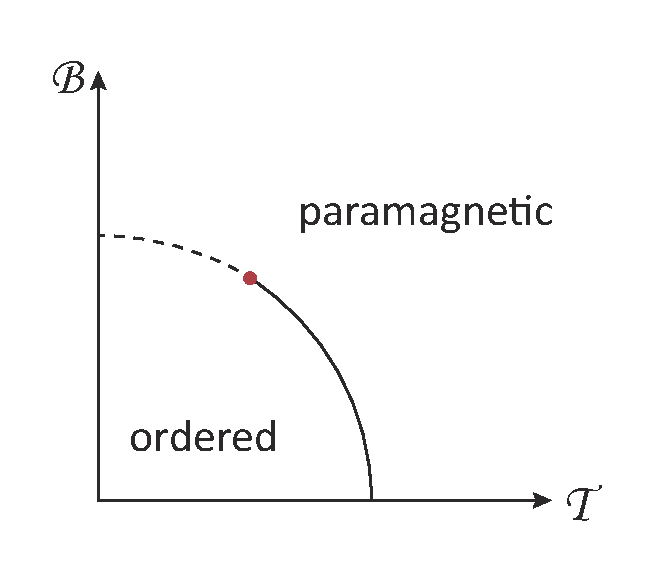
\includegraphics[width=7cm]{picture/tricritical}
\caption{Phase diagram of the tricritical Ising model. The (broken) first-order line and the (full) line of Ising critical points meet at the tricritical point $(B_t, T_t)$, shown as black dot}\label{fig:tricritical}
\end{figure}


A typical phase diagram of this model is sketched in Figure \ref{fig:tricritical}, where the lines of first-order and second-order transitions meet in the tricritical point, located at $B=B_t$ and $T=T_t$. While at a normal critical point two phases become indistinguishable, at a tricritical point three physically distinct phases merge. For that reason, this model is called the \textbf{tricritical Ising model}. The phenomenology of the tricritical Ising model is described in \cite[\S4]{cardy1996scaling}.


Remarkably, the tricritical model is described by $\cN=1$ superconformal field theory where $G$ is the supercurrent \cite[ISZ88-No.5]{friedan1985superconformal}.



\subsubsection*{3-state Potts model $(p',p)=(6,5)$}
$$\begin{array}{c| c c  c  c  } 5& 3 &{\frac{7 }{5 } } &{\frac{2 }{5 } } &{0 } \\[5pt] 4& \frac{13 }{8 } &{\frac{21 }{40 } } &{\frac{1 }{40 } } &{\frac{1 }{8 } } \\[5pt] 3&  \frac{2 }{3 } &{\frac{1 }{15 } } &{\frac{1 }{15 } } &{\frac{2 }{3 } } \\[5pt] 2& \frac{1 }{8 } &{\frac{1 }{40 } } &{\frac{21 }{40 } } &{\frac{13 }{8 } } \\[5pt] 1& 0 &{\frac{2 }{5 } } &{\frac{7 }{5 } } &{3 } \\[5pt] \hline &1&2&3&4  \end{array}$$

On a square lattice, the hamiltonian of the three-state Potts model is given by
$$\cH=- \frac{J }{2 } \sum _{x , \alpha } \left(\sigma _{x } \overline{\sigma } _{x + \alpha } + \overline{\sigma } _{x } \sigma _{x + \alpha } \right)$$
where $\sigma$ takes the values $\omega^i$ (i=1,2,3) with third root of unity $\omega=e^{2\pi i/3}$. This model undergoes a second-order phase transition at $J_c=\frac{2 }{3 } \log (\sqrt{3 } + 1)$, which is endowed with the $\bZ_3$ symmetry  \cite[ISZ88-No.12]{dotsenko1984critical}. The lattice theory is exactly solvable and consequently all critical exponents are known. For instance,
$$
h_{\sigma}=h_{\overline \sigma}=\frac1{15}~,\qquad h_\varepsilon=\frac{2}{5}~.
$$
It is tempting to identify the primary field of the unitary minimal model $\cM_{p=5}$.
However, the exact solution of the lattice model does not have operators with
conformal dimensions $\frac18$, $\frac1{40}$, $\frac{21}{40}$, and $\frac{13}8$  \cite[ISZ88-No.22]{vonGehlen:1986gk}.


In fact, the partition function of  the 3-state Potts model is described by the one of the non-diagonal type \cite[ISZ88-No.29]{Cardy:1986gw}
\be\label{3-state-Potts}
\cZ _{\text{3-Potts} }=\sum _{r=1,2 } \left\{\left| \chi _{r , 1 } + \chi _{r , 5 } \right|^{2 } + 2 \left| \chi _{r , 3 } \right|^{2 } \right\}~,
\ee
so that the primary fields are \cite[ISZ88-No.12]{dotsenko1984critical}
$$
(0,0) , \left(\frac{2 }{5 } , \frac{2 }{5 } \right) , \left(\frac{7 }{5 } , \frac{7 }{5 } \right)~, 2 \times \left(\frac{1 }{15 } , \frac{1 }{15 } \right) , 2 \times \left(\frac{2 }{3 } , \frac{2 }{3 } \right)  (0,3) , (3,0) , \left(\frac{2 }{5 } , \frac{7 }{5 } \right) , \left(\frac{7 }{5 } , \frac{2 }{5 } \right)
$$
It is noteworthy that there are chiral spin-3 current $W(z)$ and $\overline W(\overline z)$ corresponding to  (0,3), (3,0)  \cite[ISZ88-No.6]{Zamolodchikov:1985wn}. In fact, $W(z)$ with the energy momentum tensor $T(z)$ form $W_3$-algebra \cite{Fateev:1987vh}.


\subsubsection*{Other models}

It was shown in \cite[ISZ88-No.32]{Huse:1984mn} that a general unitary minimal model $\cM_p$ of diagonal type describes an RSOS model constructed in \cite[ISZ88-No.31]{Andrews:1984af}.
Furthermore, the CFT with $\bZ_k$ symmetry has been constructed in \cite[ISZ88-No.14]{fateev1985parafermionic}, which we will see in \S\ref{sec:coset}, where the central charge is
\be\label{Zk-cc} c = \frac { 2 ( k - 1 ) } { k + 2 }~.\ee
When $k=4$, the central charge is $c=1$ and the corresponding CFT is called the \textbf{Ashkin-Teller model} where the Hamiltonian is written by the two spin fields $ \sigma _ { i } $ and $ \tau _ { i } $ as
$$\mathcal { H } = - J _ { 2 } \sum _ { \langle i , j \rangle } \left( \sigma _ { i } \sigma _ { j } + \tau _ { i } \tau _ { j } \right) - J _ { 4 } \sum _ { \langle i , j \rangle } \sigma _ { i } \sigma _ { j } \tau _ { i } \tau _ { j }~.$$
The $\bZ_4$ symmetry is given by
$$
s_j\to e^{\frac{i\pi k}{2}}s_j ~, \qquad \textrm{where}\qquad
s_j\equiv \frac{\sigma _ { j } +i\tau _ { j } }{\sqrt{2}}~.
$$
This Ashkin-Teller model can be described by the free boson on an orbifold space $S^1/\bZ_2$, which will be studied in \S\ref{sec:orbif-part-funct}.
All in all, these models are main characters in the papers listed in \cite{itzykson1988conformal}.









\subsection{Conformal blocks and bootstrap}\label{sec:bootstrap}
\subsubsection*{The Operator Algebra}
The main object of a field theory is the calculation of correlation functions. We have
seen how the coordinate dependence of two- and
three-point function. We have mentioned in the
Minimal model section that one way to construct all correlation functions is to find the corresponding operator algebra:
The complete OPE (including all regular terms)
of all primary fields with each other.
Minimal model concerns about the primary fields
with its fusion rule in a theory, but doesn't tell
anything about the coefficients of operator algebra.
The goal of this section is to spell out which of
its coefficients can be fixed by conformal invariance, which are not.


We know that two-point correlation function
vanishes if the conformal dimensions of the two
fields are different. If the conformal dimensions
are the same for a finite set of primary fields
$\phi_\alpha$, the correlators are
\begin{equation}
\label{two-point-function}
\left\langle \phi _{\alpha } (w , \overline{w }) \phi _{\beta } (z , \overline{z }) \right\rangle=\frac{C _{\alpha \beta } }{(w-z)^{2 h } (\overline{w }-\overline{z })^{2 \wt{h } } }\,,
\end{equation}
where $h_\alpha=h_\beta=h$. Since the coefficients are symmetric, we are free to choose a
basis so that $C_{\alpha\beta}=\delta_{\alpha\beta}$.
Thus, conformal families associated with different
$\phi_\alpha$ are orthogonal in the sense of the
two point function.

The general form of operator algebra is given before
\eqref{op-algebra}
\begin{equation}
\label{op-alg-general}
\phi _{1 } (z , \overline{z }) \phi _{2 } (0,0)
=\sum_p \sum_{\{k,\overline k\}} C^{p\{k,\overline k\}}_{12}
z^{h _{p }-h _{1 }-h _{2 } + K } \overline{z } _{\overline{z } }^{\overline{h } _{p }-\overline{h } _{1 }-\overline{h } _{2 } + \overline{K } }
\phi^{\{k,\overline{k}\}}_p(0,0)\, ,
\end{equation}
where $h_1,h_2$ need not to be the same and
$K=\sum_i k_i$ and $\overline{K}=\sum_i \overline{k}_i$;
the expression ${k}$ means a collection of indices
$k_i$. The sum is over all the possible highest operators and its descendants, and the pre-factors
ensure the invariance under scaling transformation.

Now consider the three point function. By choosing
suitable conformal transformation, we can send two
of the coordinate to $0$ and  $\infty$. Therefore, we have
\bea
\label{3-point-function}
\left\langle \phi _{r } \left| \phi _{1 } (z , \overline{z }) \right| \phi _{2 } \right\rangle &= \lim _{w , \overline{w } \rightarrow \infty } w^{2 h _{r } }\overline{w}^{2 \overline{h } _{r } } \left\langle \phi _{r } (w , \overline{w }) \phi _{1 } (z , \overline{z }) \phi _{2 } (0,0) \right\rangle\notag\\
&= \frac{C _{r 12 } }{z^{h _{1 } + h _{2 }-h _{r } } \overline{z }^{\overline{h} _{1 } + \overline{h } _{2 }-\overline{h } _{r } } }
\eea
On the OPE side, the only contributing term is
$p\{k,\overline{k}\}=r\{0,0\}$, because of the orthogonality of the Verma modules and the comparison of pre-factors in \eqref{op-alg-general}.
We thus have
\begin{equation}
C _{12 }^{p \{0,0 \}}= C _{p 12 }
\end{equation}
which tells us that the most singular term of the
operator algebra is the coefficient of the three-point function.
Since the correlations of descendants are built on
the correlation of the primaries, we expect the
coefficient to have the form:
\begin{equation}
C^{p\{k,\overline{k}\}}_{12}=C^p_{12}
\beta^{p\{k\}}_{12}
\overline{\beta}^{p\{\overline{k}\}}_{12}\, .
\end{equation}
Holomorphic and antiholomorphic parts are separated
as usual, and by convention we set $\beta^{p\{0\}}_{ij}=1$. $\beta^{p\{k\}}_{ij}$ can be determined by BPZ equation \eqref{eq-BPZ} as functions of central charge
$c$ and of conformal dimensions.

Therefore, the only coefficients we can not determine are the coefficients $C_{pnm}$ in  the three-point functions, which must be obtained from another
source for instance through the conformal bootstrap.

\subsubsection*{Conformal Blocks}
The conformal blocks are used to build
four-point function or more. Consider a general four-point function.
\begin{equation}
\left\langle \phi _{1 } \left(z _{1 } , \overline{z } _{1 } \right) \phi _{2 } \left(z _{2 } , \overline{z } _{2 } \right) \phi _{3 } \left(z _{3 } , \overline{z } _{3 } \right) \phi _{4 } \left(z _{4 } , \overline{z } _{4 } \right) \right\rangle\,,
\end{equation}
We can perform a suitable transformation
to set $z_4 =0, z_1=\infty, z_2=1$ and $z_3 =x$ so as to reduce 4 variables to only $x$. The correlation function we want calculate becomes:
\begin{equation}
G _{34 }^{21 } (x , \overline{x }) =
\lim _{z _{1 } , \overline{z } _{1 } \rightarrow \infty } z _{1 }^{2 h _{1 } } \overline{z } _{1 }^{2\overline{h} _{1 } } \left\langle \phi _{1 } \left(z _{1 } , \overline{z } _{1 } \right) \phi _{2 } (1,1) \phi _{3 } (x , \overline{x }) \phi _{4 } (0,0) \right\rangle\, ,
\end{equation}
where the order in which the indices of $G$ appear
is important.
Applying the operator algebra \eqref{op-alg-general} to
$\phi_3(x,\overline{x})\phi_4(0,0)$ ,
the function $G^{21}_{34}$ becomes
\begin{equation}
G _{34 }^{21 } (x , \overline{x })=\sum _{p } C _{34 }^{p } C _{12 }^{p } \mathcal{F } _{34 }^{21 } (p | x) \overline{\mathcal{F } } _{34 }^{21 } (p | \overline{x })\, ,
\end{equation}
where
\begin{equation}
\label{conformal-block}
\mathcal{F } _{34 }^{21 } (p | x)=x^{h _{p }-h _{3 }-h _{4 } } \sum _{\{k \} } \beta _{34 }^{p (k) } x^{K } \frac{\left\langle h _{1 } \left| \phi _{2 } (1) L _{- k _{1 } } \cdots L _{- k _{N } } \right| h _{p } \right\rangle }{\left\langle h _{1 } \left| \phi _{2 } (1) \right| h _{p } \right\rangle }\, ,
\end{equation}
which are called conformal blocks. The denominator
is simply equal to $(C^p_{21})^{1/2}$. They can
be simply calculated by commuting the Virasoro
generators over the field $\phi_2(1)$, and can
be represented in terms of central charge and
conformal dimensions. Since we combine $\phi_3$ and $\phi_4$ to produce intermediate operator $[\phi_p]$, and $[\phi_p]$ then interacts with
$\phi_1$ and $\phi_2$, this process can be displayed in diagrammatic language. More precisely, the diagram shows in Fig. \ref{fig:tree} corresponds to $\mathcal{F } _{i j }^{\ell m } (p | x) \overline{\mathcal{F } } _{i j }^{\ell m } (p | \overline{x })$.
\begin{figure}[ht]
	\centering
	\includegraphics[width=0.4\linewidth]{picture/tree}
	\caption{Diagram for the conformal block}
	\label{fig:tree}
\end{figure}
One may write the conformal block as a power
series in $x$:
\begin{equation}
\mathcal{F } _{34 }^{21 } (p | x)=x^{h _{p }-h _{3 }-h _{4 } } \sum _{K=0 }^{\infty } \mathcal{F } _{K } x^{K }\,.
\end{equation}
and list several leading coefficients in the
above series which can be calculated by
\eqref{conformal-block}.
\begin{equation}
\mathcal{F}_{0}=1\, , \qquad
\mathcal{F } _{1 }=\frac{\left(h _{p } + h _{2 }-h _{1 } \right) \left(h _{p } + h _{3 }-h _{4 } \right) }{2 h _{p } }
\end{equation}
\bea
\mathcal{F } _{2 } &= \frac{\left(h _{p } + h _{2 }-h _{1 } \right) \left(h _{p } + h _{2 }-h _{1 } + 1 \right) \left(h + h _{3 }-h _{4 } \right) \left(h + h _{3 }-h _{4 } + 1 \right) }{4 h _{p } \left(2 h _{p } + 1 \right) }\notag\\
&+ 2 \left(\frac{h _{1 } + h _{2 } }{2 } + \frac{h _{p } \left(h _{p }-1 \right) }{2 \left(2 h _{p } + 1 \right) }-\frac{3 \left(h _{1 }-h _{2 } \right)^{2 } }{2 \left(2 h _{p } + 1 \right) } \right)^{2 }\notag\\
&
\times \left(\frac{h _{3 } + h _{4 } }{2 } + \frac{h _{p } \left(h _{p }-1 \right) }{2 \left(2 h _{p } + 1 \right) }-\frac{3 \left(h _{3 }-h _{4 } \right)^{2 } }{2 \left(2 h _{p } + 1 \right) } \right)^{2 } \left(c + \frac{2 h _{p } \left(8 h _{p }-5 \right) }{2 h _{p } + 1 } \right)^{- 1 }
\eea

\subsubsection*{Crossing Symmetry and
the Conformal Bootstrap}
In defining the function $G^{21}_{24}(x,\overline{x})$,
we have chosen a specific order for the
four fields $\phi_{1-4}$ within the correlation
function. By using different conformal transformation as before, we can send $z_2$ to $0$ and $z_4$
to $1$, and then $z_3$ proves to be $1-x$. We combine $\phi_2$ and
$\phi_3$ at first in the calculation process, thus
get the same answer. Therefore, we obtain the
following identity.
\begin{equation}
\label{Bootstrap method}
G^{21}_{34}(x,\overline{x})=G^{41}_{32}(1-x,1-\overline{x})
\, .
\end{equation}
or more precisely
\begin{equation}\label{bootstrap}
\sum _{p } C _{21 }^{p } C _{34 }^{p } \mathcal{F } _{34 }^{21 } (p | x) \overline{\mathcal{F } } _{34 }^{21 } (p | \overline{x })=
\sum _{q } C _{41 }^{q } C _{32 }^{q } \mathcal{F } _{32 }^{41 } (q | 1-x) \overline{\mathcal{F } } _{32 }^{41 } (q | 1-\overline{x })
\end{equation}
This relation is represented graphically on Fig.\ref{fig:crossing-symmetry}

\begin{figure}[ht]
	\centering
	\includegraphics[width=0.8\linewidth]{picture/crossing-symmetry}
	\caption{Crossing symmetry}
	\label{fig:crossing-symmetry}
\end{figure}

If the conformal block $\mathcal{F}$ is known, then \eqref{Bootstrap method} yields a system of equations that
can determine $C_{ijk}$'s and $h,\overline{h}$'s. The program of calculating the correlation functions simply by assuming crossing
symmetry is known as the bootstrap approach. For minimal models, the bootstrap equations can be solved completely.


\end{document}
